\section{Theoretische Grundlagen}
\subsection{Bandstrukturen}
Bandstrukturen in Kristallen sind dadurch zu erklären, dass sich die Atomorbitale der einzelnen Atome überlagern. Aus den diskreten Energieniveaus der einzelnen Atome werden so Energiebänder. Dieses Modell nennt man auch ``tight binding''. Ein anderes Modell genannt ``plane wave expansion'' nimmt an, dass die Elektronen im Kristall quasi frei sind und so durch ausgedehnte Wellen beschrieben werden können. Die Dispersionsrelation wird aber durch die Gitterstruktur verändert und so entstehen Energiebänder, die so Bandlücken in die eigentlich verbundene Energieverteilung bringen.

Anhand der Besetzung dieser Energiebänder lassen sich Materialien in drei unterschiedliche Kategorien bezüglich der Leitfähigkeit einordnen. Denn ein Material leitet nur, wenn das energetisch höchste Energieband nur teilweise besetzt ist. Im Gegensatz zu diesen Metallen haben die Isolatoren zwischen dem letzten besetzten Energieband (Valenzband) und dem nächsten unbesetzten Energieband (Leitungsband) eine Bandlücke, die von den Elektronen normalerweise nicht überwunden werden kann. Bei den Halbleitern ist diese Bandlücke besonders klein, sodass Elektronen beispielsweise durch thermische Anregung in das Leitungsband gelangen können. Die Größe der Energielücken für Halbleiter ist im Bereich von einigen Zehntel eV.

Intrinsische Halbleiter sind Halbleiter, die keine Fehlstellen oder Fremdatome haben und dennoch durch elektronische Anregungen leitfähig werden können. Um nun die Konzentration der Elektronen im Leitungsband zu berechnen nutzt man die Beziehung
\begin{equation}
\frac{N}{V}=n = 2\cdot \int_{E_L}^\infty D_L(E)\cdot f(E)dE
\end{equation}
mit der Fermi-Verteilung $f(E)$ und der Zustandsdichte im Leitungsband $D_L(E)$.
Analog findet man die Beziehung für die Konzentration der Löcher im Valenzband:
\begin{equation}
 \frac{P}{V}=p = 2\cdot \int_{E_V}^\infty D_V(E)\cdot [1-f(E)]dE
\end{equation}
Dazu muss gesagt werden, dass Löcher im Valenzband einfach fehlende Elektronen darstellen. Sie entstehen, indem Elektronen angeregt werden und aus dem Valenzband ins Leitungsband gehen. Das Konzept des Lochs ist wichtig, weil sie auch zum Ladungstransport beitragen, indem die anderen Valenzelektronen in die Löcher nachrücken. Effektiv bewegt sich dann das Loch und transportiert so positive Ladung.

Für die Dispersionsrelation für Elektronen im Leitungsband bzw. Löcher im Valenzband wird
\begin{equation}
 E(\vec k)= E_L + \frac{\hbar}{2}\cdot \left(\frac{k_x^2}{m^*_{xx}}\cdot \frac{k_y^2}{m^*_{yy}}\cdot\frac{k_z^2}{m^*_{zz}} \right)
\end{equation}
angenommen und dies führt im Fall isotroper effektiver Massen zu den Zustandsdichten
\begin{eqnarray}
 D_L(E)&=&\frac{1}{4\pi^2}\left(\frac{2m_n^*}{\hbar^2}\right)^\frac{3}{2}(E-E_L)^\frac{1}{2},\;\; E>E_L\\
 D_V(E)&=&\frac{1}{4\pi^2}\left(\frac{2m_p^*}{\hbar^2}\right)^\frac{3}{2}(E_V-E)^\frac{1}{2},\;\; E_V>E.
\end{eqnarray}


\subsection{Dotierung von Halbleitern}
Die Ladungsträgerkonzentrationen sind in den meisten Halbleitern zu niedrig, um bei
Raumtemperatur eine nennenswerte Leitfähigkeit zu liefern. Die Situation lässt sich
ändern, indem man eine sehr kleine Menge elektrisch aktiver Störstellen (Fremdatome)
in den Halbleiter einbringt. Diesen Prozess nennt man Dotierung. Die Fremdatome
ändern die Leitfähigkeit, indem sie entweder Elektronen in das Leitungsband abgeben
oder Elektronen aus dem Valenzband aufnehmen, also Löcher erzeugen. Dementsprechend
nennt man sie auch Elektronendonator bzw. Elektronenakzeptor. Es gibt zwei Arten von Dotierungen in einem Halbleiter. n-Dotierung nennt man das
Einbringen von Störstellenatomen (Donatoren), die freie Elektronen in das Leitungsband
abgeben. Als p-Dotierung bezeichnet man das Einbringen von Störstellenatomen
(Akzeptoren), die freie Löcher im Valenzband erzeugen.
Bei der n-Dotierung werden dagegen fünfwertige Donatoratome wie P, As oder Sb in das
Si-Gitter eingebracht, vergleiche hierzu Abbildung \ref{Dotierung}.

Eine wichtige Kenngröße für Halbleiter ist die intrinsische Ladungsträgerdichte und die Ladungsträgerverteilung. Diese sind maßgeblich für die sogenannte Eigenleitung, daher die Leitfähigkeit der Halbleiter abhängig der Temperatur. Wie oben beschrieben, können Elektronen erst durch Energieanregung ins Leitungsband „springen“ und somit als Ladungsträger zur Verfügung stehen. Wenn man äußere Anregungen vernachlässigt, hängt dich intrinsische Ladungsträgerdichte also sehr stark von der Temperatur ab, da die Elektronen nur durch thermische Anregungen Energie erhalten können. Die intrinsische Ladungsträgerdichte bleibt daher bis zu einer gewissen Temperatur quasi null, da die thermischen Anregungen aufgrund der Temperatur nicht groß genug sind, um die Bandlücke zu überwinden.  In Abbildung \ref{Leitung} stellt die gestrichelte Kurve den Verlauf der intrinsischen Ladungsträgerdichte im Leitungsband dar. Im Falle von dotierten Halbleitern (durchgezogene Linie), tragen zunächst die durch die Fremdatome eingebrachten Ladungsträger zur konstanten Ladungsträgerdichte bei, bis die thermischen Anregungen hier auch zum Tragen kommen.

\begin{figure}[htbp]  
     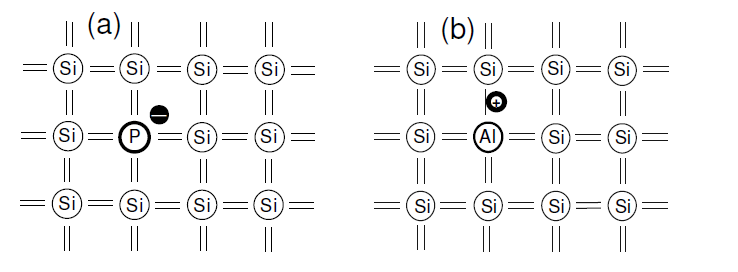
\includegraphics[width=0.7\textwidth]{Dotierung.png}
  \caption{n- und p-Dotierung im Si-Kristall \cite{Hofmann}}
  \label{Dotierung}
\end{figure}

\begin{figure}[htbp]  
     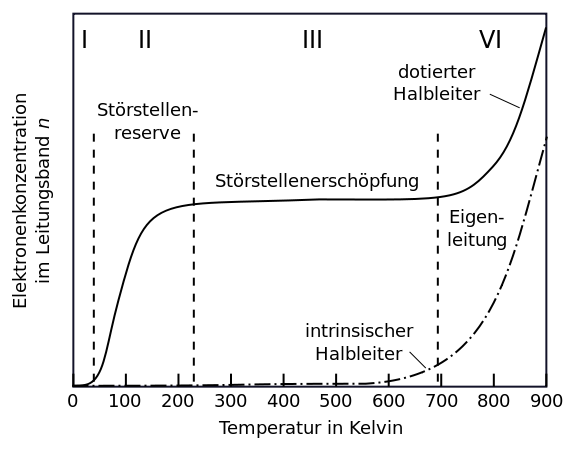
\includegraphics[width=0.7\textwidth]{Leitung.png}
  \caption{Ladungsträgerdichte im Leitungsband abhängig der Temperatur \cite{Leitung}}
\label{Leitung}
\end{figure}

\subsection{Ladungstransport in Halbleitern}

Ein bekanntes Modell für den Ladungstransport in Halbleitern ist das Drude-Modell. Dieses betrachtet die Bewegungen von Elektronen durch ein Kristallgitter als Abfolge von Stößen mit den Kristallionen. Dabei werden die Stoßvorgänge durch eine mittlere Stoßzeit, in der sich das Elektron frei im Kristall bewegt, und einer sog. Driftgeschwindigkeit beschrieben. Die Driftgeschwindigkeit bezeichnet dabei die Geschwindigkeit des Elektrons, welche ausschließlich durch ein angelegtes elektrisches Feld erzeugt wird. Thermische Beiträge zur Elektron-Geschwindigkeit werden hier nicht berücksichtigt. Mit der bekannten elektrischen Kraft auf ein Elektron im elektrischen Feld ergibt sich folgende 
Bewegungsgleichung:

\begin{equation}
\frac{m_e}{\tau}v_D = -eE
\end{equation}

mit der Driftgeschwindigkeit $v_D$ und der mittleren Stoßzeit $\tau$. Über diesen Zusammenhang zwischen Driftgeschwindigkeit und angelegtem elektrischen Feld kann man die sog. Beweglichkeit $\mu$ definieren:

\begin{equation}
\mu = \frac{v_D}{E}= \frac{e\tau}{m_e}
\end{equation}

Im allgemeinen beschreibt das Drude-Modell die Elektronen eines Halbleiters als Elektronengas, in dem alle Elektronen zur Leitung beitragen. 

\subsection{Hall-Effekt}
Der Hall Effekt tritt auf, wenn in einem Leiter oder einem Halbleiter senkrecht zu einem Magnetfeld $\vec B$ ein Strom fließt. Die Lorentzkraft
\begin{equation}
 m_e\frac{\mathrm d v}{\mathrm d t}= -e(\vec E + \vec v \times \vec B)
\end{equation}
lenkt dann die Ladungsträger so ab, dass ein elektrisches Feld $E_H$ entsteht, das zu Magnetfeld $B$ und Strom $j_x$ senkrecht steht. Im Folgenden fließe der angelegte Strom in x-Richtung, das Hall-Feld zeige in y-Richtung und das Magnetfeld in z-Richtung. Nun definiert man die Hall-Konstante durch 
\begin{equation}
 R_H=\frac{E_H}{j_x\cdot B}.
\end{equation}

$j$ wird durch die Konzentrationen $n,p$ und die Driftgeschwindigkeiten $v_e, v_h$ der Löcher und Elektronen ausgedrückt:
\begin{equation}
 \vec j=-ne\vec v_e+pe\vec v_h
\end{equation}
und wiederum die Driftgeschwindigkeiten durch 
\begin{eqnarray}
 v_x^e &=& -\mu_eE_x+\mu_e\omega_e\tau_eE_H\\
 v_x^h &=& +\mu_hE_x+\mu_h\omega_h\tau_hE_H\\
 v_y^e &=& -\mu_eE_H-\mu_e\omega_e\tau_eE_x\\
 v_y^h &=& +\mu_hE_H-\mu_h\omega_h\tau_hE_x.
\end{eqnarray}
Dabei sind die $\mu$ die Beweglichkeiten der Löcher bzw. Elektronen, die $\omega=\frac{eB}{m}$ die Zyklotronfrequenzen und die $\tau$ die Relaxationszeiten der Elektronen bzw. Löcher. Dabei  wurden Terme der Ordnung $\omega^2$ vernachlässigt, was äquivalent zur Vernachlässigung des Magnetoresistiven Effekts ist. Der Magnetoresistive Effekt bezeichnet das Ändern des elektrischen Widerstands eines Materials durch Anlegen eines Magnetfelds.

Setzt man nun den statischen Fall als Voraussetzung, ist also $j_y=0$, dann ergibt sich durch Einsetzen der Driftgeschwindigkeiten und elektrischer Felder die Hall-Konstante zu
\begin{equation}
 R_H = \frac{1}{e}\cdot\frac{p-n\left(\frac{\mu_e}{\mu_h}\right)^2}{\left(p+n\frac{\mu_e}{\mu_h}\right)^2}
\end{equation}
